%%%%%%%%%%%%%%%%%%%%%%% file manuscript.tex %%%%%%%%%%%%%%%%%%%%%%%
%%%%%%%%%%%%%%%%%%%%%%%%%%%%%%%%%%%%%%%%%%%%%%%%%%%%%%%%%%%%%%%%%%%
%
\RequirePackage{fix-cm}
%\documentclass{svjour3}
\documentclass[twocolumn]{svjour3}          % twocolumn
\usepackage{natbib}
\usepackage{breakcites}
\usepackage{graphicx}
\usepackage{mathptmx}      % use Times fonts if available on your TeX system
\usepackage{hyperref}

\journalname{Psychonomic Bulletin \& Review}

\begin{document}

\title{Category Learning Effects on Memory
  %\thanks{Grants or other notes
  %about the article that should go on the front page should be
  %placed here. General acknowledgments should be placed at the end of the article.}
}

%\subtitle{}
%\titlerunning{Short form of title}

\author{Kevin O'Neill \and Audrey Liu \and Siyuan Yin \and Timothy Brady \and Felipe De~Brigard}
%\authorrunning{Short form of author list} % if too long for running head

\institute{K. O'Neill \at
  Center for Cognitive Neuroscience \\
  Duke University \\
  \email{kevin.oneill@duke.edu}
}

\date{Received: date / Accepted: date}
% The correct dates will be entered by the editor


\maketitle

\begin{abstract}
Category learning...
\keywords{First keyword \and Second keyword \and More}
\end{abstract}

\section*{Introduction}
\label{intro}

\section*{Methods}
\label{methods}

\textbf{Participants }
%\subsection*{Participants}
%\label{methods:participants}
867 participants were recruited via Amazon Mechanical Turk
(\url{https://www.mturk.com}). All participants were from the United
States, had at least 100 approved hits, had an overall hit approval
rate of at least 95\%, and received $\$2.00$ compensation for their
participation. Data from 133 participants were excluded because of
failure to learn the assigned category below 85\% accuracy during the
last 20 trials of learning (a benchmark used in \cite{DeBrigard2017}),
or excessive response time (greater than the mean + three standard
deviations, XX seconds), so data were analyzed with the remaining 733
individuals. All participants were provided informed consent in
accordance with the Duke University IRB.

\noindent\textbf{Materials }
%\subsection*{Materials}
%\label{methods:materials}
Stimuli consisted of MATLAB (2018b)-generated flowers, used previously
in \citet{DeBrigard2017}. These flowers vary over five features, with
each feature having three possible values: number of petals (four,
six, or eight), petal color (blue, green or yellow), center shape
(circle, triangle, or square), center color (orange, purple, or
turquoise), and number of sepals (one, two, or three). Figure
\ref{fig:flowers} demonstrates three flowers that encapsulate all
possible values of the five features. All flowers were displayed on
the center of the screen with a white background.

\begin{figure}
  
\includegraphics[scale=0.15]{flower1.png}
  
\includegraphics[scale=0.15]{flower2.png}
  
\includegraphics[scale=0.15]{flower3.png}
  \caption{Example stimuli encompassing the range of values for each
    feature.  From left to right: 4 blue petals, orange circle center,
    1 sepal; 6 green petals, purple triangle center, 2 sepals; and 8
    yellow petals, blue square center, 3 sepals. See more
    \citet{DeBrigard2017} for further details.}
  \label{fig:flowers}
\end{figure}

\noindent\textbf{Procedure }
%\subsection*{Procedure}
%\label{methods:procedure}
Procedure followed Experiment 4 of \citet{DeBrigard2017}, with a few
revisions. This paradigm includes a learning, study, and test
phase. Participants began the experiment by reading an instruction
screen for a minimum of 30 seconds which detailed the five stimulus
features and the possible values those features could take. This
instruction screen also displayed two example stimuli for
illustration. Participants were instructed that they would see flowers
on the screen, one at a time, and were asked to determine whether each
flower belonged to the species \emph{avlonia}.  Participants were told
that \emph{avlonias} differed from other flowers in one simple way
(e.g., only \emph{avlonias} have four petals), but that they must
discover what makes \emph{avlonia} flowers unique. Participants were
told that they must initially guess, but that they would eventually
learn what makes a flower an \emph{avlonia}. Crucially, the feature
and value that constituted and \emph{avlonia} was counterbalanced
across participants. During each of the three phases of the
experiment, each value of each feature was displayed in 1/3 of the
trials for that phase, so that the co-occurrence of all feature/value
combinations was uniform. In this way, 1/3 of all flowers presented
were members of the learned category (\emph{avlonia}). Participants
were also assigned a not-learned category, constituted by a value of a
different feature, of which they were unaware. The not-learned
category was never mentioned to the participants, statistically
independent of the learned category, and counterbalanced across
participants.

In addition to the category manipulations in \citet{DeBrigard2017}, we
introducted two further manipulations on learning: whether the
participant was explicitly instructed of the the learned category's
discriminating feature and value or not (instruction), and whether the
participant actively categorized flowers during learning, or merely
watched the screen categorize the flowers as \emph{avlonias} or
not-\emph{avlonias} (practice). These factors were manipulated fully
between-subjects.

First, participants learned to categorize flowers into the species
\emph{avlonia}. For the practiced condition, participants completed 72
self-paced trials in which they pressed the ``y'' key if the flower
was an avlonia, or the ``n'' key otherwise. Immediate feedback
(``Correct'' or ``Incorrect'') was presented after each key-press for
1s. For the not-practiced condition, participants passively viewed 72
trials in which a flower was shown for 3s, and a categorization
(``Avlonia'' or ``Not Avlonia'') was presented immediately after for
1s. Of the 72 flowers presented, 16 flowers were in the learned
category but not the not-learned category, 16 flowers were in the
not-learned category but not the learned category, 8 flowers were in
both categories, and 32 flowers were in neither category.

In the study phase, participants were asked to memorize 18
flowers. Each flower was shown for 5s following a 1s inter-trial
interval. None of these flowers were shown previously in the learning
phase. Of these 18 flowers, 4 flowers were in the learned category but
not the not-learned category, 4 flowers were in the not-learned
category but not the learned category, 2 flowers were in both
categories, and 8 flowers were in neither category. Participants were
told that they would receive a bonus if they could remember a high
number of flowers (XX participants were in fact given a $\$X.XX$ bonus
for a hit rate exceeding 85\%).

Finally, in the test phase, participants were told that they would see
54 flowers, one by one, and asked to press the ``y'' key if the flower
was old (presented during the study phase), or to press the ``n'' key
otherwise. Each trial was self-paced with a 1s inter-trial
interval. Of these 54 flowers, 18 were presented during study. Of the
remaining 36 flowers (lures), 8 flowers were in the learned category
but not the not-learned category, 8 flowers were in the not-learned
category but not the learned category, 4 flowers were in both
categories, and 16 flowers were in neither category. None of the lures
appeared in the learning or study phases.

\section*{Results}
\label{results}

\noindent\textbf{Learning }
%\subsection*{Learning}
%\label{results:learning}
Because participants in the not-practiced condition did not make any
responses during learning, we limit this analysis to participants in
the practiced condition. As found in \citet{DeBrigard2017},
participants in the not-instructed condition started at near chance
(64.31\%) categorization accuracy in the first 20 trials, and
gradually rose to 86.15\% accuraccy in the last 20 trials. In
contrast, partipants in the instructed condition began at 82.42\%
accuracy, and gradually rose to 89.00\% accuracy. This confirms that
explicit instruction allowed participants to successfully learn the
\emph{avlonia} category before practice.

\begin{figure}
  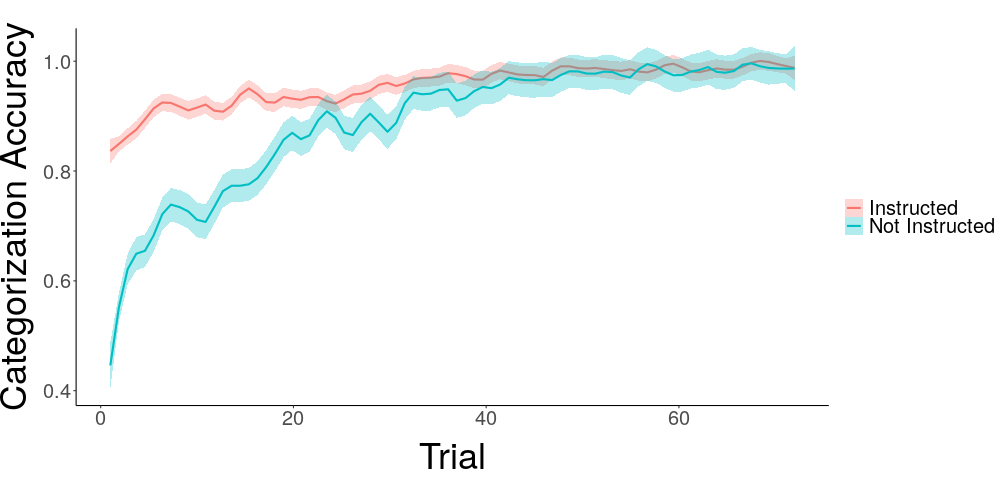
\includegraphics[width=0.5\textwidth]{learning.png}
  \caption{Learning curves for participants in the practiced
    condition.}
  \label{fig:learning}
\end{figure}

\noindent\textbf{Memory Performance }
%\subsection*{Memory Performance}
%\label{results:memory}

\begin{figure}
  %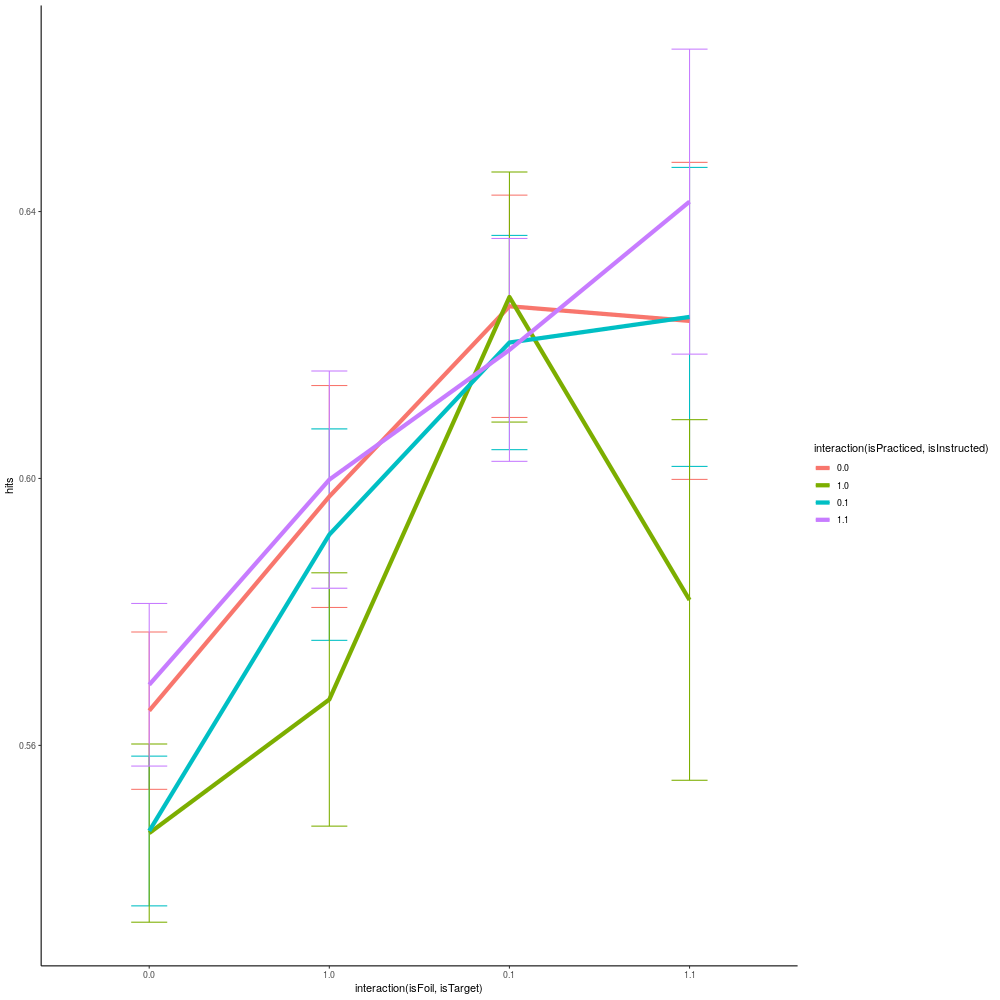
\includegraphics[width=0.5\textwidth]{E6_hits.png}
  \caption{Hit rates.}
  \label{fig:hits}
\end{figure}

\begin{figure}
  %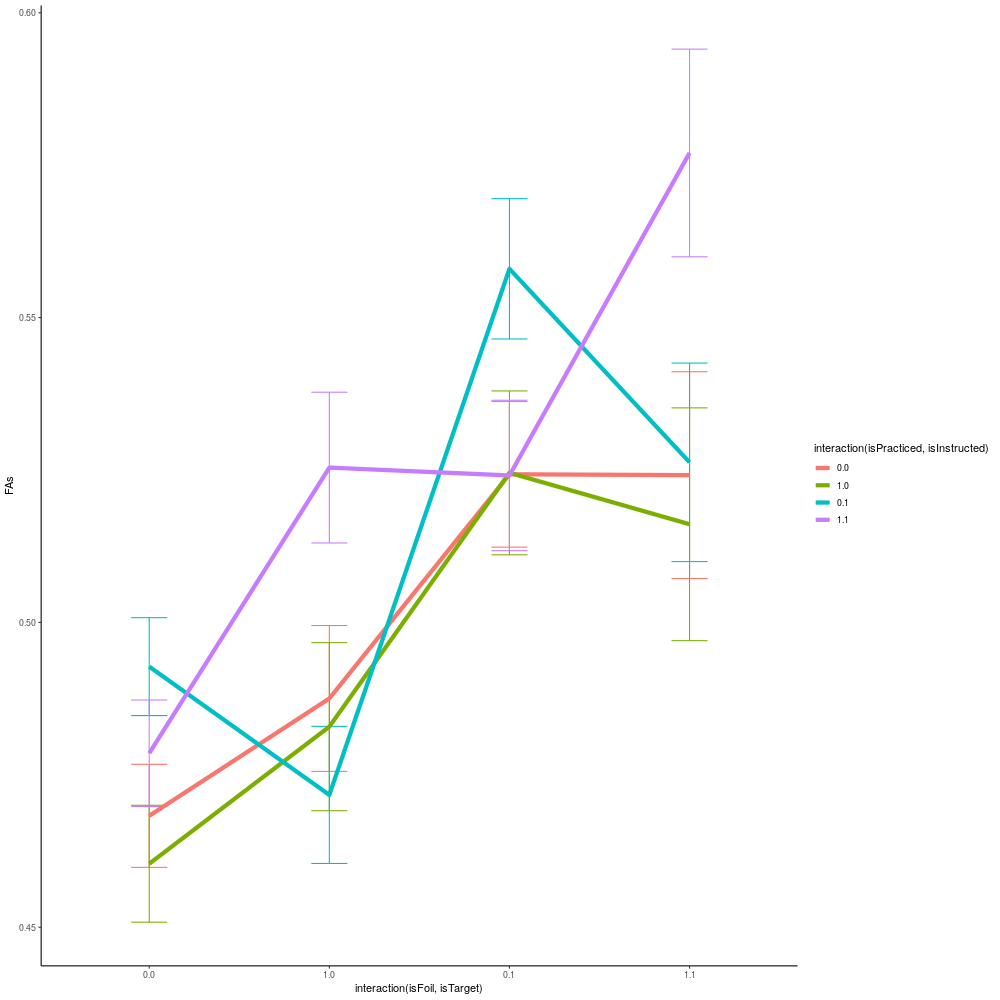
\includegraphics[width=0.5\textwidth]{E6_FAs.png}
  \caption{False alarm rates.}
  \label{fig:fas}
\end{figure}

\noindent\textbf{Signal Detection Theory }
%\subsection*{Signal Detection Theory}
%\label{results:sdt}


\begin{figure}
  %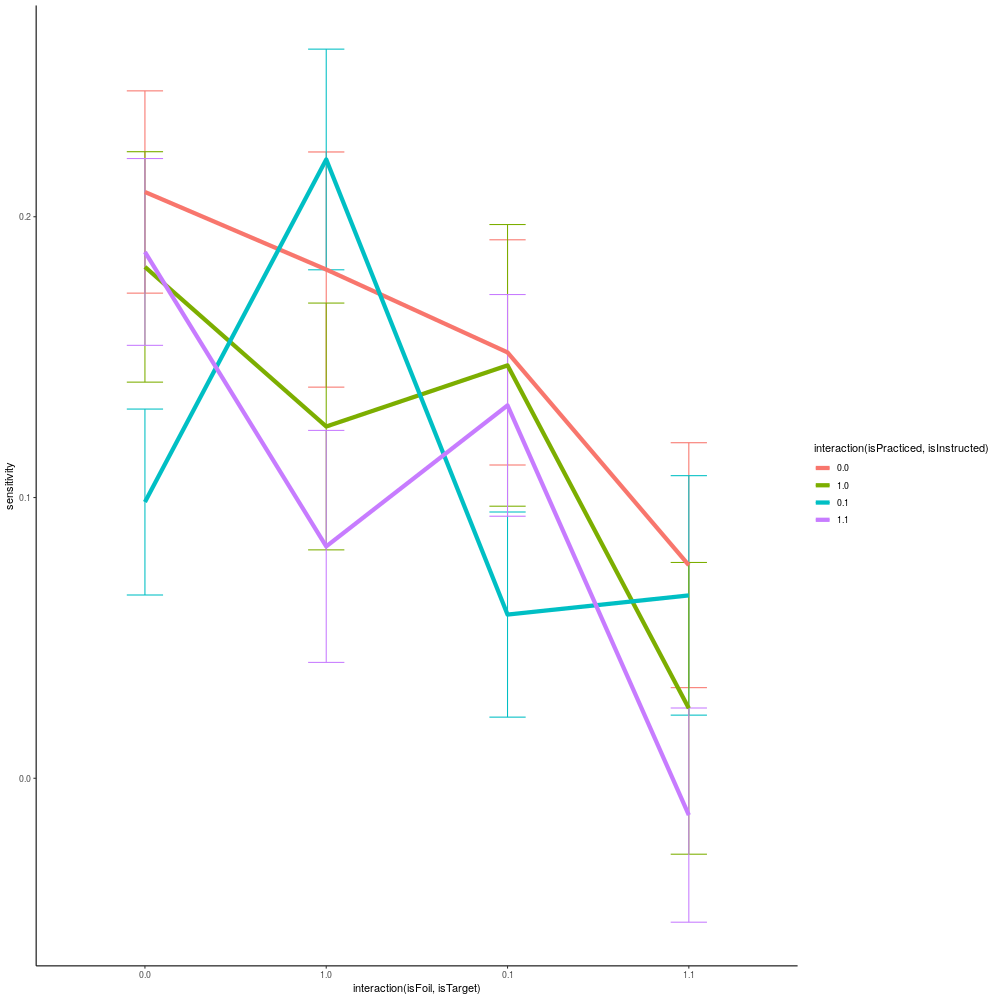
\includegraphics[width=0.5\textwidth]{E6_sensitivity.png}
  \caption{Sensitivity.}
  \label{fig:sensitivity}
\end{figure}

\begin{figure}
  %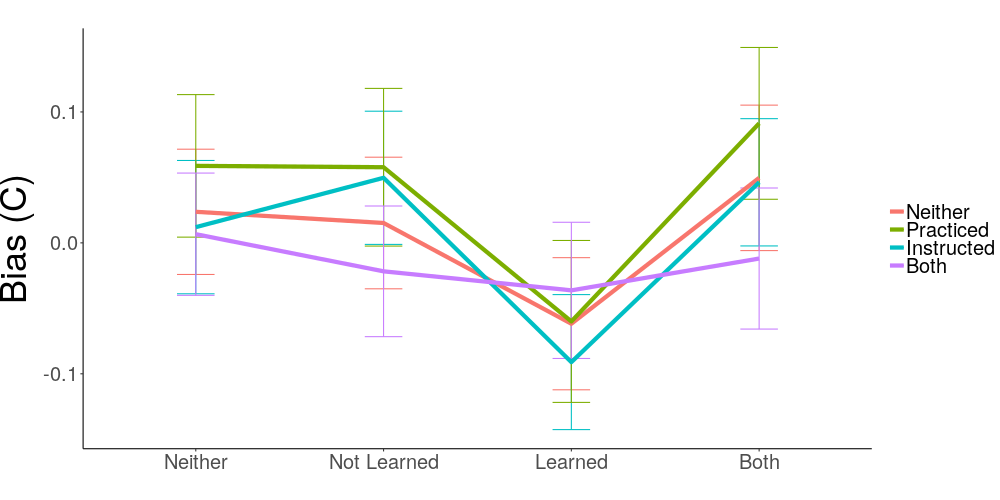
\includegraphics[width=0.5\textwidth]{E6_bias.png}
  \caption{Bias.}
  \label{fig:learning}
\end{figure}

\section*{Discussion}
\label{discussion}

\begin{acknowledgements}
\end{acknowledgements}

\bibliographystyle{spbasic} \bibliography{category_learning}

\end{document}

